\documentclass[a4paper,oneside]{article}
\usepackage{indentfirst}
\usepackage{graphicx}
\usepackage{newtxtext,newtxmath}
\usepackage[top=0.7in, bottom=0.7in, left = 0.7in, right = 0.7in]{geometry}
\usepackage{enumitem}
\usepackage{caption}
\setlist{nolistsep}
\setlength{\belowcaptionskip}{-10pt}
\begin{document}
\title{\vspace{-0.7in}Term Project Proposal\\
High-Grade Prostate Cancer Prediction using DNA Methylation Data}
\author{Tanjung Dion (201899213)\\Fawwaz Dzaky Zakiyal (201899213)\\}
\date{Bioinformatics (Fall 2018)}
\maketitle
 
\section{Introduction}
Prostate cancer is a disease that affects a significant proportion of the male population, but in most cases, the disease is harmless. However, for the small portion of the population with high-grade prostate cancer, the
disease can be extremely debilitating, causing painful symptoms and even death. Prior studies have been performed, showing how hereditary factors, alcohol consumption, sexual activity, family history and race can each play a role in developing high-grade PCa. Over the past years rapid advances in next-generation sequencing technology has led to the timely advent of The Cancer Genome Atlas (TCGA) project which provides the most comprehensive genomic data for various kinds of cancer. In the previous research indicates classification of patient samples using TCGA Exon expression or SNP datasets. However, recent study show that DNA methylation act as better bio-markers and help in improving the cancer prognosis \cite{one}.

\section{Vocabulary}
\begin{itemize}
\item \textbf{DNA methylation}: the process of adding methyl groups to DNA, in this process modification of covalent nucleotides in the human genome, namely cytosine and also guanine. It is one form of epigenetic modification which take an important role in the development of cancer.
\item \textbf{Gleason Score}: a measure (from 2-10) of the aggression of prostate cancer cells based on clinical pathology of prostate tissue.
\item \textbf{High-Grade Prostate Cancer (HGPCa)}: a form of prostate cancer that is likely to metastasize and generally results in poor patient outcomes mortality, complications, and long-term disease free survival). A gleason score from 8-10 is indicative of High-Grade prostate cancer, while scores below 8 are considered not as severe.
\end{itemize}


\section{Methodology}
\subsection{Dataset}
The data used in this paper is publicly available through the National Cancer Institute GDC Data Portal, and can be found online under Project TCGA-PRAD. This data set consists of genomic information and clinical pathology reports belonging to roughly 500 patients who have been diagnosed with prostate cancer (a Gleason Score anywhere between 2 to 10). It contains of both clinical (recurrence, survival \& treatment resistance) and molecular profiles (Exon (mRNA) expression, DNA methylation, Copy Number Variations (CNV) \& Single Nucleotide Polymorphism (SNP)) for both tumor samples and normal controls. Data from TCGA has improved the ability of oncologists to diagnose, treat, and prevent cancer through a better understanding of the genetic basis of this disease. The clinical pathology reports were also critical for our analysis because they contain the Gleason scores for each patient, which allows us to determine whether a patient has HGPCa \cite{two}. The dataset detail can be seen at Figure \ref{fig:dataset_detail}.

\begin{figure}
  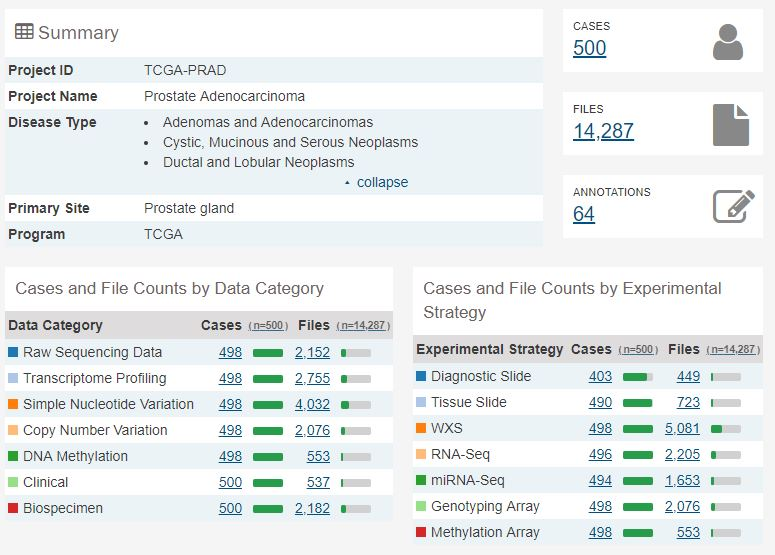
\includegraphics[width=0.7\linewidth]{dataset_detail}
  \centering
  \caption{Dataset Detail}
  \label{fig:dataset_detail}
\end{figure}

\subsection{System Design}
The process consist of data preprocessing of TCGA-PRAD dataset, and continue with feature selection of extracted DNA methylation data. After that, training the classifier models, testing and evaluating those models. The system design can be seen at Figure \ref{fig:system_design}.

\begin{figure}
  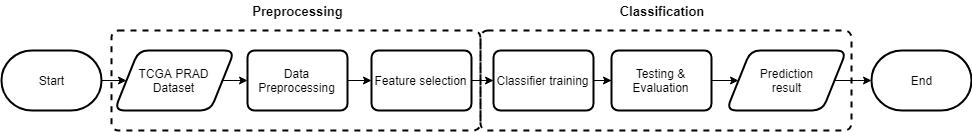
\includegraphics[width=0.9\linewidth]{system_design}
  \centering
  \caption{System Design}
  \label{fig:system_design}
\end{figure}

\subsection{Preprocessing}
Significant amounts of pre-processing needed to be performed in our to make the data usable in any way. First, we had to consolidate our data across hundreds of clinical pathology reports and DNA methylation profiles. After consolidation, we constructed a feature matrix in which each row corresponds to a patient and each column corresponds to a DNA methylation.
\par
We will also applied the adjustments described below to each column in order to normalize our data and using Principal Component Analysis (PCA) as feature selection algorithm to eliminate the useless DNA methylation and reduce the search space.
\subsection{Classifier Algorithms}

Perform a classification for cancer prediction :
\begin{enumerate}
\item K-Nearest Neighbor (KNN)
\item Support Vector Machine (SVM)
\item Multilayer Perceptron (MLP)
\end{enumerate}

\subsection{Testing \& Evaluation}
This project will finding a model that has the maximum classification accuracy, given by the Equation \ref{eq:1}, where $y_{i}'$ is the predicted label for instance $i$, $y$ is the true label for instance $i$. $I$ is an indicator function, if the statement is true, it will return $1$, and vice-versa.

\begin{equation} \label{eq:1}
accuracy =  \frac{1}{n}  \sum_{i=1}^n  I(y_{i}' = y_{i})
\end{equation}




\begin{thebibliography}{1}
\bibitem{one} Hao, Xiaoke, et al. {\em DNA methylation markers for diagnosis and prognosis of common cancers.} Proceedings of the National Academy of Sciences 114.28 (2017): 7414-7419.
\bibitem{two} GDC. Portal.Gdc.Cancer.Gov, 2018, {\em https://portal.gdc.cancer.gov/projects/TCGA-PRAD.} Accessed 2 Nov 2018.
\bibitem{three} Ang, Jun Chin, et al. {\em Supervised, unsupervised, and semi-supervised feature selection: a review on gene selection.} IEEE-ACM transactions on computational biology and bioinformatics 13.5 (2016): 971-989.
\end{thebibliography}
\end{document}